\documentclass[10pt, a4paper]{article}
\usepackage[utf8]{inputenc}
\usepackage[T1]{fontenc}
\usepackage{bigints,bbm,slashed,mathtools,amssymb,amsmath,amsfonts,amsthm}
\usepackage{tikz}
\usepackage{tikz-cd}
\usepackage{pgfplots}
\pgfplotsset{compat=1.16}
\usetikzlibrary{babel}
\usetikzlibrary{positioning,arrows}
\usetikzlibrary{decorations.pathreplacing}
\usetikzlibrary{patterns}
\usepackage{tikzsymbols}
\usepackage[T1]{fontenc}
\usepackage[utf8]{inputenc}

\begin{document}

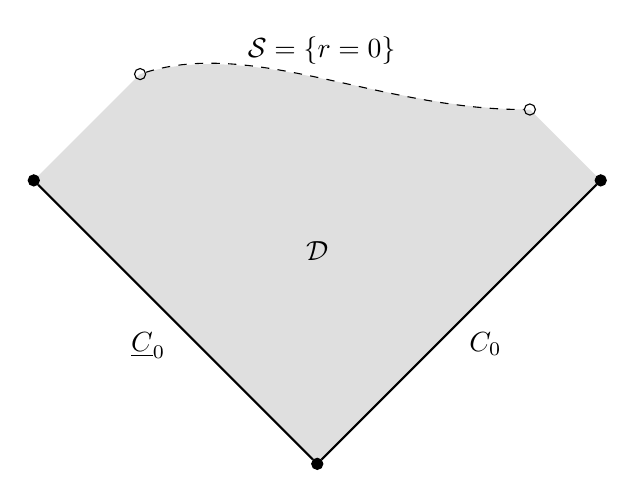
\begin{tikzpicture}[scale=0.9]
        \path[fill=lightgray, opacity=0.5] (0, -4) -- (-4, 0) -- (-2.5, 1.5)
            .. controls (-0.9, 2) and (0.9, 1) .. (3, 1)
            -- (4, 0) -- (0, -4);

        \node (p) at (0, -4) [circle, draw, inner sep=0.5mm, fill=black] {};
        \node (r) at (4, 0) [circle, draw, inner sep=0.5mm, fill=black] {};
        \node (l) at (-4, 0) [circle, draw, inner sep=0.5mm, fill=black] {};
        \node (rs) at (3, 1) [circle, draw, inner sep=0.5mm] {};
        \node (ls) at (-2.5, 1.5) [circle, draw, inner sep=0.5mm] {};

        \node at (0, -1) {$\mathcal{D}$};

        \draw [thick] (p) -- (r)
            node [midway, below right] {$C_0$};
        \draw [thick] (p) -- (l)
            node [midway, below left] {$\underline{C}_0$};
        \draw [dashed] (ls) .. controls (-0.9, 2) and (0.9, 1) .. (rs)
            node [midway, above=0.5mm] {$\mathcal{S} = \{ r = 0 \}$};
    \end{tikzpicture}

\end{document}